\chapter{مصر باستان}

به نقطه‌ی آغاز سفر خوش آمدید. بیایید سری به موزه‌ی بریتانیا بزنیم تا یک متن کهن را ببینیم، پاپیروس ریاضی رایند%
\LTRfootnote{ Rhind Mathematical Papyrus}.
قدمت این پاپیروس به حدود ۱۵۵۰ سال پیش از میلاد می‌رسد و متعلق به مصر باستان است. نترسید، نمی‌خواهیم الآن آن را بخوانیم! فقط جالب است بدانید با چه عبارتی شروع می‌شود. «محاسبه‌ی دقیق؛ راهیابی به دانش همه‌ی چیزهای موجود و شناخت همه‌ی رازها و اسرار نهفته.»
\begin{figure}[h]
	\centering
	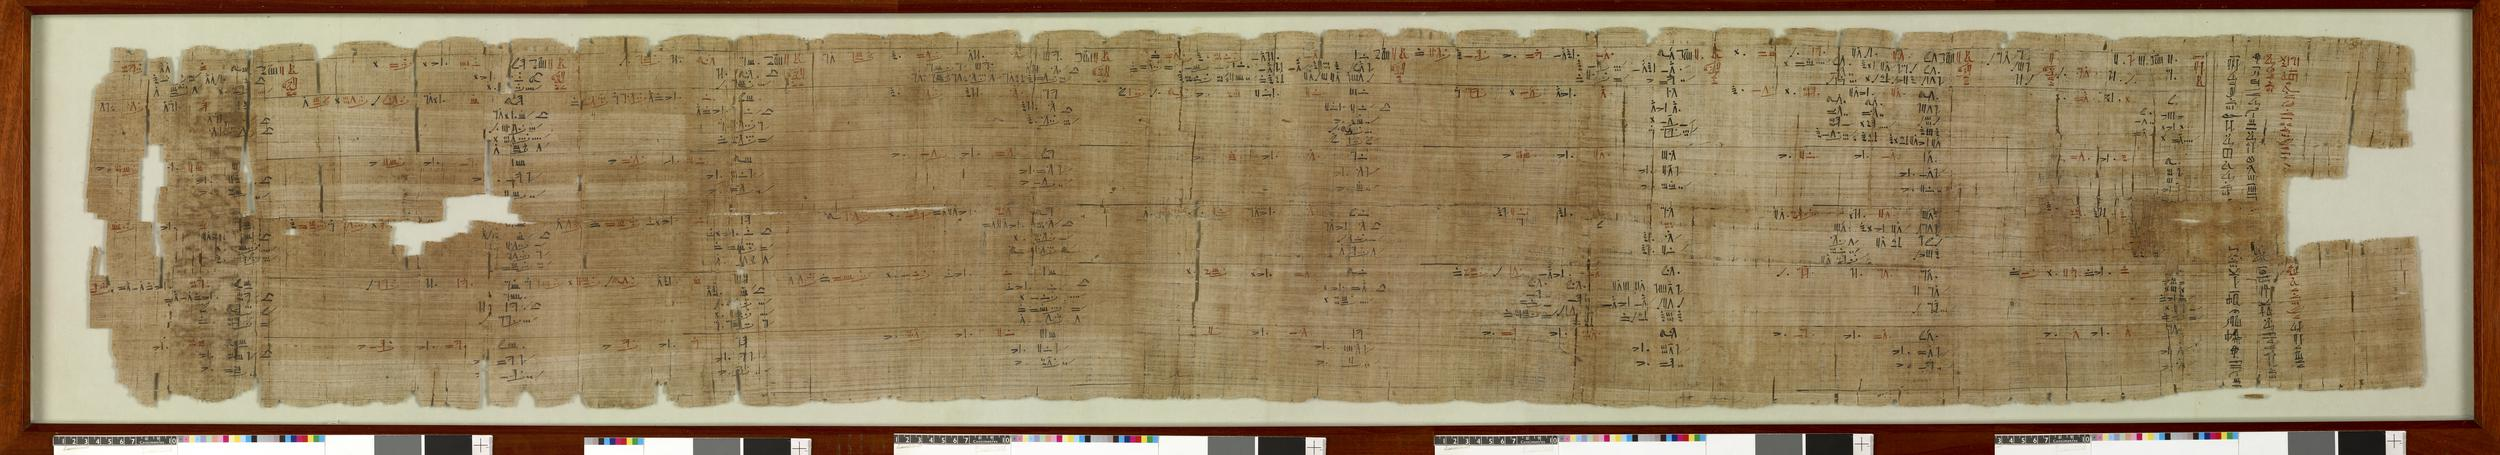
\includegraphics[width=\textwidth]{./Images/366139001.jpg}
	\caption{پاپیروس ریاضی رایند}
	\label{fig1.1}
\end{figure}

%%%%%%%%%%%%%%%%%%%%%%%%%%%%%%%%%%%%%%%%%%%%%%
\section{سیستم‌های عددی و محاسبات}

کمی عقب‌تر برویم، به ۳۱۰۰ سال پیش از میلاد. نوشتار در مصر تقریباً در همین دوران آغاز شد و بیشتر نوشته‌های اولیه به حسابداری و ثبت انواع کالاها مربوط می‌شد. از همان ابتدای پیدایش خط در مصر، دو سبک نوشتاری وجود داشت: خط هیروگلیف برای نوشتن معمولاً روی دیوارها و ستون‌ها و تندیس‌ها و خط هیراتیک برای نوشتن روزمره معمولاً روی پاپیروس. بنابراین مصری‌ها دو سیستم عددنویسی مختلف نیز داشتند، سیستم هیروگلیف و سیستم هیراتیک. در سیستم هیروگلیف هر توان ۱۰ با یک نماد نشان داده می‌شود.
\begin{figure}[h]
	\centering
	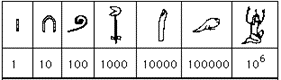
\includegraphics[width=0.5\textwidth]{./Images/Hieroglyph.png}
	\caption{سیستم عددنویسی هیروگلیف}
	\label{fig1.2}
\end{figure}

اما اعداد در سیستم هیروگلیف چطور نوشته می‌شوند؟ نظرتان چیست که خودتان کشف کنید؟ من سه تا تصویر واقعی نشان شما می‌دهم و شما به کمک شکل \ref{fig1.2} تلاش کنید که بفهمید هر کدام چه عددی را نشان می‌دهند.
\begin{figure}[h]
	\centering
	\begin{subfigure}{0.3\textwidth}
		\centering
		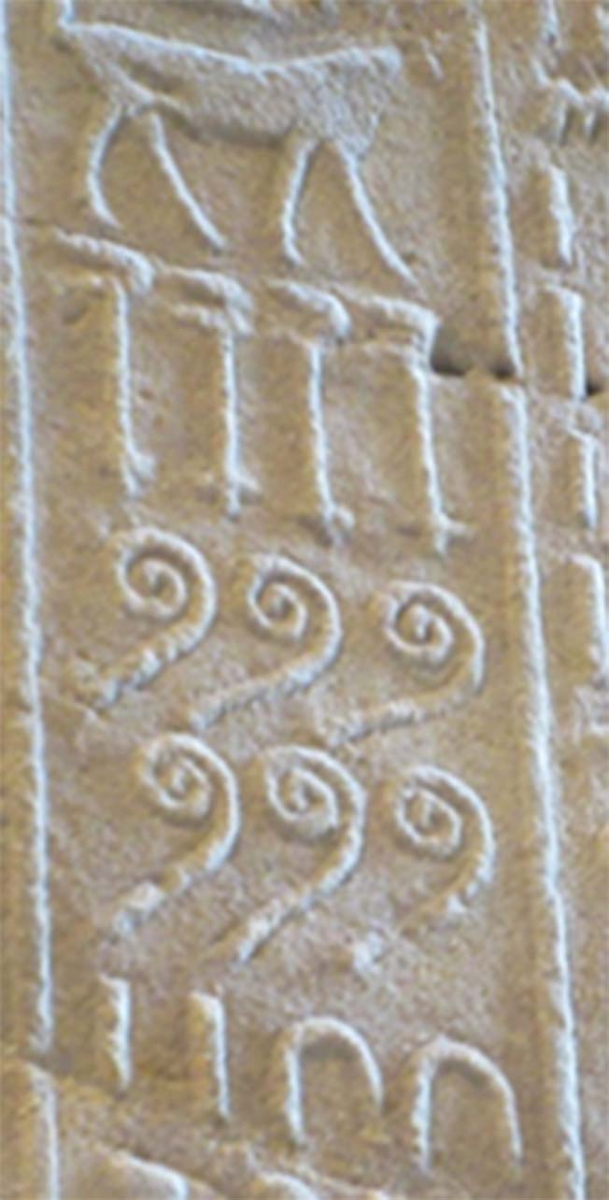
\includegraphics[height=2in, keepaspectratio=true]{./Images/Huffman_Egypt-Fig5-Louvre.jpg}
		\caption{لوور}
		\label{fig1.3.1}
	\end{subfigure}
	\hspace{0.03\textwidth}
	\begin{subfigure}{0.3\textwidth}
		\centering
		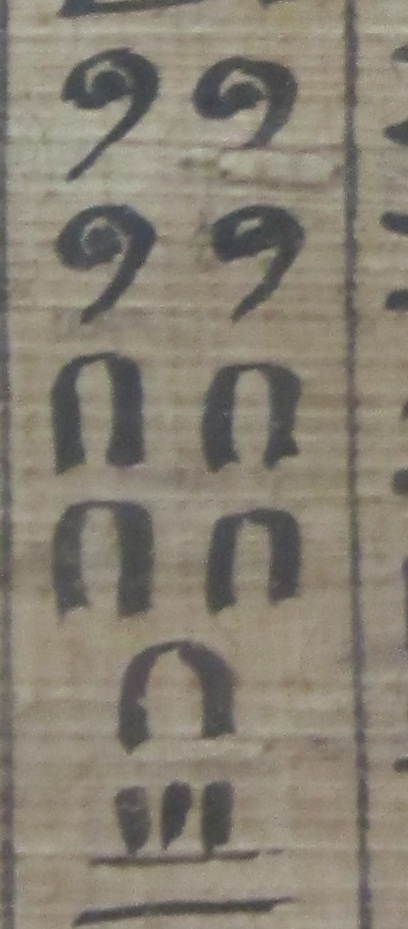
\includegraphics[height=2in, keepaspectratio=true]{./Images/Huffman_Egypt-Fig6b-Turin.jpg}
		\caption{تورین}
		\label{fig1.3.2}
	\end{subfigure}
	\hspace{0.03\textwidth}
	\begin{subfigure}{0.3\textwidth}
		\centering
		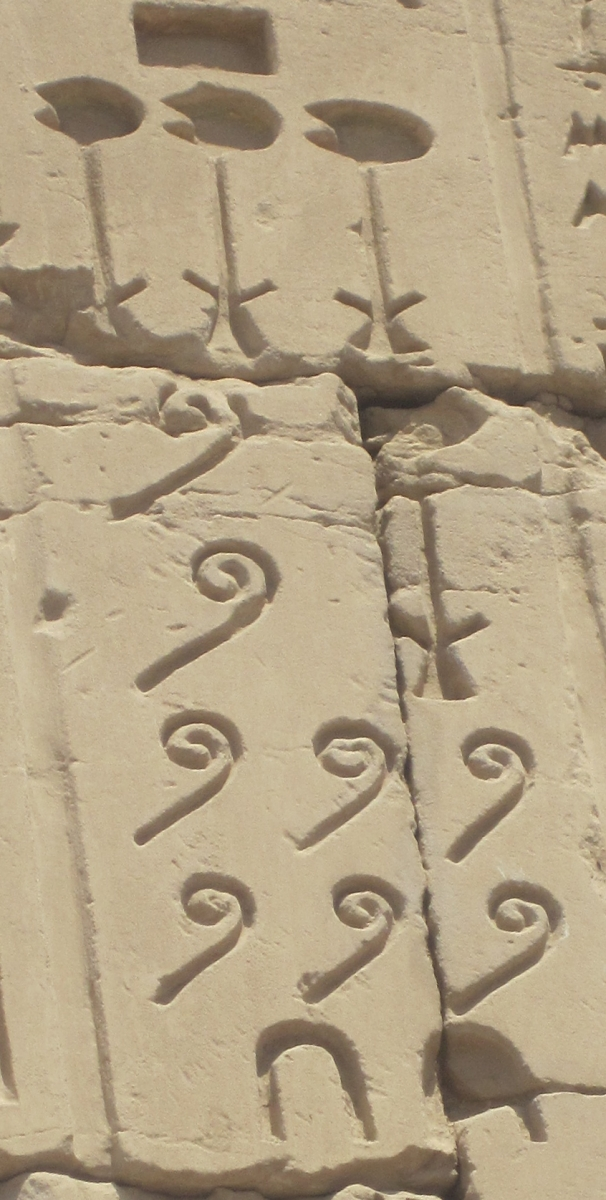
\includegraphics[height=2in, keepaspectratio=true]{./Images/Huffman_Egypt-Fig7a-Karnak.jpg}
		\caption{کارنک}
		\label{fig1.3.3}
	\end{subfigure}
	
	\caption{نمونه‌ی هیروگلیف‌های عددی}
	\label{fig1.3}
\end{figure}

شکل \ref{fig1.3} شامل سه متن هیروگلیف مختلف است. تصویر سمت راست، مربوط به سال‌نامه‌ی توتمس سوم در معبد کارنَک در شهر الأقصر مصر است که اکنون در موزه‌ی لوور شهر پاریس نگهداری می‌شود و عدد ۴۶۲۲ را نمایش می‌دهد. تصویر وسط، مربوط به یک پاپیروس است که در شهر تورین ایتالیا نگهداری می‌شود و عدد ۴۵۳ را نمایش می‌دهد. تصویر سمت چپ، دیواری در معبد کارنک است که عدد ۴۸۲۰ را نمایش می‌دهد. آیا به راز آن‌ها پی بردید؟ کافی است تعداد هر نماد را بشمارید تا رقم مربوط به هر جایگاه را بیابید. به ترتیب قرار گرفتن نمادها نیز دقت کنید. نماد توان بزرگتر، بالاتر یا در سمت راست قرار می‌گیرد. همچنین، نوشته را از بالا به پایین یا از راست به چپ می‌نویسند. حالا می‌توانید دو عدد ۷۸۳ و ۲۷۵ را در سیستم هیروگلیف بنویسید؟

سیستم هیراتیک روش متفاوتی برای عددنویسی دارد. در این سیستم، هر رقم ۱ تا ۹ نماد خاصی دارد. همچنین، هر عدد مضرب ۱۰ از ۱۰ تا ۹۰، هر عدد مضرب ۱۰۰ از ۱۰۰ تا ۹۰۰ و ... هر کدام دارای نماد خاصی هستند. برای مثال، برای نوشتن عدد ۳۷ کافی است ۳۰ و ۷ را کنار هم بنویسیم.
\begin{figure}[h]
	\centering
	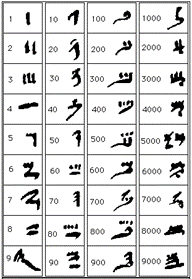
\includegraphics[width=0.4\textwidth]{./Images/Hieratic.png}
	\caption{سیستم عددنویسی هیراتیک}
	\label{fig1.4}
\end{figure}

خب تا اینجای سفر چطور بود؟ امیدوارم اوایلش خسته‌کننده نباشد، چون با مفاهیم ابتدایی سروکار داریم. به دو عمل جمع و تفریق نمی‌پردازیم چون کار آسانی است. خودتان امتحان کنید. دو عدد ۷۸۳ و ۲۷۵ را که نوشته بودید، یک بار با هم جمع کنید و یک بار از هم کم کنید. حال به سراغ ضرب و تقسیم می‌رویم که دیگر به راحتی جمع و تفریق نیست.

الگوریتم مصری برای ضرب بر پایه‌ی فرایند دو برابر کردن متوالی است. بگذارید با یک مثال توضیح دهم. فرض کنید می‌خواهیم ۱۲ را در ۱۳ ضرب کنیم. یک جدول دو ستونی تشکیل می‌دهیم و ۱ و ۱۲ را در ردیف اول می‌نویسیم. حال هر کدام را در ۲ ضرب می‌کنیم و در ردیف بعدی می‌نویسیم. به محض این‌که عدد سمت چپ مساوی ۱۳ یا بزرگتر شد، فرایند را متوقف می‌کنیم و آن ردیف را حذف می‌کنیم. حال با عددهای ستون چپ، عدد ۱۳ را می‌سازیم، یعنی با جمع ۱، ۴ و ۸. سپس عدد متناظر هر کدام در ستون راست را با هم جمع می‌کنیم، یعنی ۱۲، ۴۸ و ۹۶ که جمعشان برابر با ۱۵۶ می‌شود. به حاصل ۱۲ ضرب در ۱۳ رسیدیم.



%%%%%%%%%%%%%%%%%%%%%%%%%%%%%%%%%%%%%%%%%%%%%%
\section{معادلات خطی و استدلال تناسبی}

بر اساس پاپیروس‌های رایند و مسکو می‌دانیم که مصری‌ها با مسائلی مواجه بودند که ما امروزه آن‌ها را معادلات خطی، تناسب‌ها، و هندسه می‌نامیم.